\documentclass[11pt,a4paper]{article}
\usepackage[utf8]{inputenc}
\usepackage[T1]{fontenc}
\usepackage{tgpagella}
\usepackage[spanish]{babel}
\usepackage{geometry}
\usepackage{booktabs}
\usepackage{xcolor}
\usepackage{titlesec}
\usepackage{fancyhdr}
\usepackage[parfill]{parskip}
\usepackage[expansion=false]{microtype}
\usepackage{hyperref}
\usepackage{setspace}
\usepackage{needspace}
\usepackage{graphicx}
\widowpenalty=10000
\clubpenalty=10000
\displaywidowpenalty=10000

\geometry{top=3.0cm,bottom=3.0cm,left=3.5cm,right=3.5cm}
\setlength{\parskip}{0.65em}
\setlength{\parindent}{0em}

\definecolor{azulai}{RGB}{30,80,140}
\definecolor{doradoai}{RGB}{140,90,0}
\definecolor{grisai}{RGB}{70,70,70}

\titleformat{\section}{\Large\bfseries\color{azulai}}{}{0em}{}[{\color{azulai}\titlerule[0.5pt]}]
\titlespacing*{\section}{0pt}{1.8em}{0.8em}
\titleformat{\subsection}{\large\bfseries\color{doradoai}}{}{0em}{}
\titlespacing*{\subsection}{0pt}{1.4em}{0.5em}
\titleformat{\subsubsection}{\normalsize\bfseries\color{grisai}}{}{0em}{}
\titlespacing*{\subsubsection}{0pt}{1.0em}{0.3em}

\pagestyle{fancy}\fancyhf{}
\rhead{\textcolor{grisai}{\small Izas — Arquitectura Interna}}
\lhead{\textcolor{grisai}{\small Sol · Ascendente · Nodos}}
\cfoot{\textcolor{grisai}{\small\thepage}}
\renewcommand{\headrulewidth}{0.3pt}

\hypersetup{colorlinks=true,linkcolor=azulai,urlcolor=azulai}
\setstretch{1.45}
\tolerance=1500
\emergencystretch=4em

\begin{document}

% ── Portada ──────────────────────────────────────────────────────────────────
\begin{titlepage}
  \centering
  \vspace*{1.5cm}
  {\Huge\bfseries\color{azulai} Sol · Ascendente · Nodos}\\[0.5cm]
  {\large\color{grisai} Arquitectura Interna}\\[0.3cm]
  {\small\itshape\color{grisai} Dirección vital, punto de entrada y eje de desarrollo}\\[2cm]
  {\huge\color{doradoai} Izas}\\[1.5cm]
  {\Large 16/04/1979 \quad 04:20}\\[0.3cm]
  {\Large Pamplona, España}\\[0.3cm]
  {\normalsize Lat: 42.8157° \quad Lon: -1.6522° \quad UTC+02:00}\\[0.3cm]
  {\normalsize Ascendente: Acuario 6°20' \quad
    MC: Escorpio 29°12'}\\[2cm]
  \begin{tabular}{lll}
    \textbf{Sol:} & Aries & Casa 2 \\
    \textbf{Ascendente:} & Acuario & Punto de entrada principal: Urano \\
    \textbf{Nodo Norte:} & Virgo & Casa 7 \\
    \textbf{Nodo Sur:}   & Piscis & Casa 1 \\
  \end{tabular}\\[2cm]
  \vfill
  {\small Generado el 19/05/2026}
\end{titlepage}

\tableofcontents
\newpage

% ── Datos de referencia ───────────────────────────────────────────────────────
\section{Datos de referencia}

\begin{center}
\begin{tabular}{llll}
  \toprule
  \textbf{Punto} & \textbf{Signo} & \textbf{Casa} & \textbf{Posición} \\
  \midrule
  Sol           & Aries & 2 & 25°31' \\
  Ascendente    & Acuario & --- & 6°20' \\
  Medio Cielo   & Escorpio & --- & 29°12' \\
  Nodo Norte    & Virgo & 7 & 16°50' \\
  Nodo Sur      & Piscis & 1 & 16°50' \\
  \bottomrule
\end{tabular}
\end{center}

\vspace{0.5cm}
\textbf{Regente del Ascendente (Acuario):} 
Urano —
Escorpio, 
Casa 9

\vspace{0.5cm}
\textbf{Aspectos entre Sol, Ascendente y Nodos:}

\vspace{0.3cm}
\textit{No aparecen aspectos directos entre Sol, Ascendente y Nodos dentro de los orbes definidos. Esto no significa ausencia de relación entre estos puntos, sino que la lectura se apoya principalmente en sus signos, casas, elementos e integración general.}

\needspace{3\baselineskip}
\subsection*{Grados sensibles}

El Medio Cielo está en grado anaretico de Escorpio. Esto señala una zona sensible de orientación: puede haber una sensación de cierre, culminación o exigencia especial en la manera en que este eje se expresa.

\vspace{0.7cm}

\begin{center}
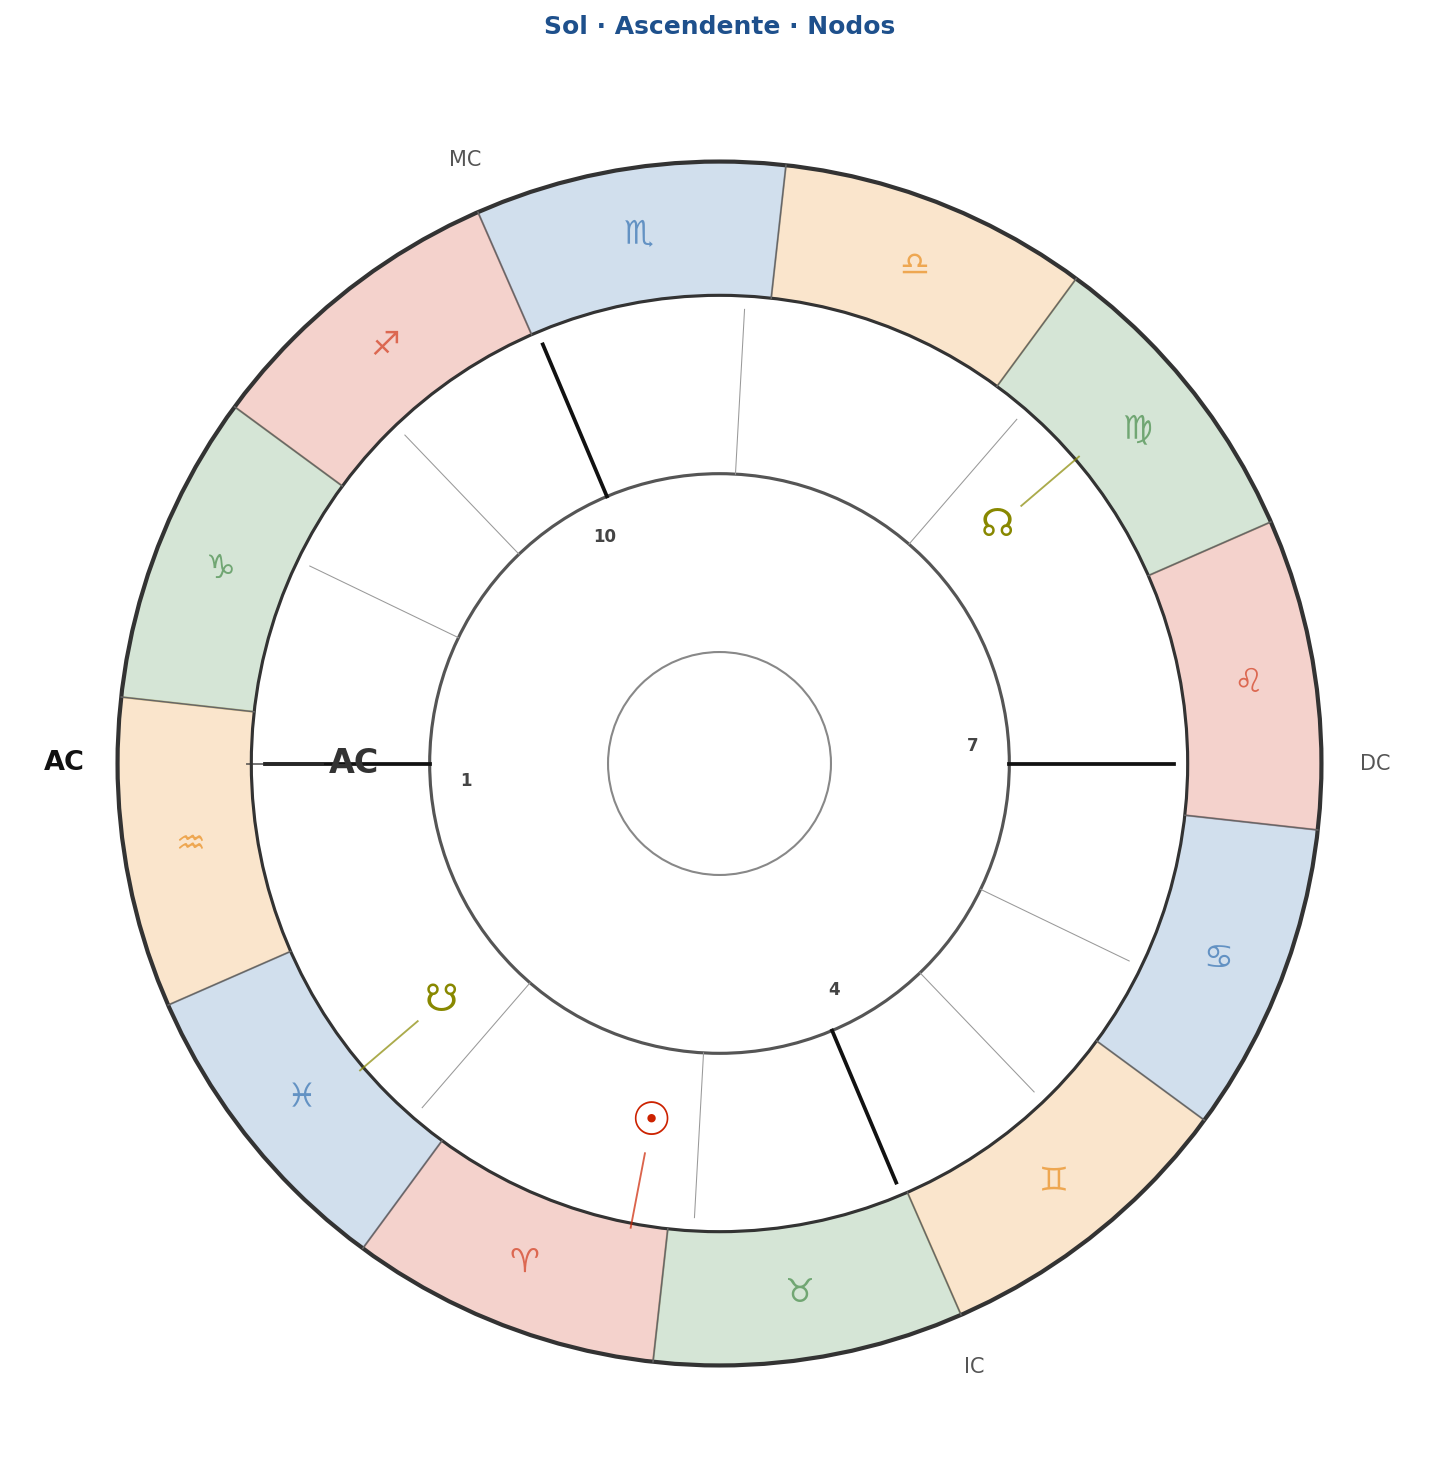
\includegraphics[width=0.72\textwidth]{Izas_Sol_ASC_Nodos_rueda.png}
\end{center}


\vspace{0.3cm}
\Needspace{5\baselineskip}

% ── Interpretación ────────────────────────────────────────────────────────────
\section{Interpretación — Arquitectura Interna}

\begin{center}
{\small\itshape
No se trata de definir quién eres. Se trata de observar cómo se organiza tu dirección,
cómo atraviesas la vida y qué tensión influye en tu forma de avanzar.
}
\end{center}

\vspace{0.5cm}
\Needspace{5\baselineskip}


% ── 1. Dirección general ──────────────────────────────────────────────────────
\needspace{3\baselineskip}
\subsection{1. Dirección general}

El Sol está en Aries, Casa 2. El Ascendente está en Acuario. El Nodo Norte está en Virgo, Casa 7, y el Nodo Sur en Piscis, Casa 1.

El Sol en Aries y el Ascendente en Acuario pertenecen a elementos compatibles. Esto puede ayudar a que tu manera de reaccionar y tu dirección principal se apoyen con cierta fluidez.

El Sol en Aries, Casa 2, no tiene un aspecto directo con los Nodos. La tensión entre el Nodo Norte en Virgo, Casa 7, y el Nodo Sur en Piscis, Casa 1, se expresa de una forma más independiente respecto a la dirección solar.

\vspace{0.5cm}
\Needspace{5\baselineskip}


% ── 2. Sol ────────────────────────────────────────────────────────────────────
\needspace{3\baselineskip}
\subsection{2. El Sol — Dirección principal}

\needspace{3\baselineskip}
\subsubsection*{Sol en Aries · Casa 2}

Tu dirección se activa cuando puedes empezar algo. Necesitas movimiento, iniciativa y la sensación de que hay un objetivo hacia el que avanzar. Cuando pasas demasiado tiempo esperando, conteniéndote o sin poder actuar, la energía empieza a acumularse y suele salir en forma de irritación, impulsividad o agotamiento.

No suele faltarte impulso. Lo difícil aparece cuando arrancas demasiado rápido, sin suficiente base o sin tener claro qué quieres sostener realmente. Puedes empezar muchas cosas con fuerza y perder conexión con ellas a mitad de camino.

Te desgasta sentir que no puedes avanzar, depender constantemente del ritmo de otras personas o tener que esperar demasiado para actuar. Cuando no encuentras una dirección clara, es fácil acabar moviéndote por tensión más que por verdadera decisión.

Tu dirección se fortalece cuando desarrollas algo propio y estable. Necesitas construir recursos, capacidades o formas de sostenerte que puedas reconocer como tuyas.

La sensación de dependencia constante, inestabilidad o falta de valor personal suele desgastarte profundamente. Te ayuda avanzar poco a poco, consolidando lo que haces y viendo resultados concretos.

Cuando no puedes apoyarte en algo sólido, es fácil perder motivación o sentir que toda la energía se dispersa.
El Sol está en Aries interceptado, en Casa 2. Esto puede hacer que la dirección solar no salga de forma inmediata o evidente. La fuerza está, pero puede necesitar más tiempo, más consciencia y mejores condiciones para expresarse con claridad. No indica ausencia de dirección, sino una dirección que requiere ser desbloqueada poco a poco y llevada a la vida de una forma más deliberada.

\vspace{0.5cm}
\Needspace{5\baselineskip}


% ── 3. Ascendente ─────────────────────────────────────────────────────────────
\needspace{3\baselineskip}
\subsection{3. El Ascendente — Forma de relacionarte con la vida}

\needspace{3\baselineskip}
\subsubsection*{Acuario · Regente: Urano}

Muchas veces necesitas entender lo que ocurre antes de conectar emocionalmente con ello. Tu mente suele intentar ordenar, observar o encontrar perspectiva antes de reaccionar.

Cuando el entorno exige respuestas emocionales inmediatas o demasiado intensas, es fácil que te alejes hacia la observación y parezcas más distante de lo que realmente estás.

Te ayuda tener espacio para pensar, comprender y encontrar tu propia forma de relacionarte con lo que vives.

El regente del Ascendente es Urano, situado en Escorpio, Casa 9. Urano pertenece a un elemento con una lógica diferente a la del Ascendente. Esto puede hacer que vivas las cosas de una forma, mientras otra parte de ti necesita orientarse desde un ritmo completamente diferente.. La Casa 9 muestra un territorio importante desde el que organizas tu forma de entrar en la vida.

\vspace{0.5cm}
\Needspace{5\baselineskip}


% ── 4. Nodos ──────────────────────────────────────────────────────────────────
\needspace{3\baselineskip}
\subsection{4. Nodo Norte y Nodo Sur — Dirección de crecimiento}

\needspace{3\baselineskip}
\subsubsection*{Nodo Norte en Virgo · Casa 7 \\
Nodo Sur en Piscis · Casa 1}

Tu dirección pide orden, claridad y capacidad de distinguir qué funciona realmente para ti. Aprender a poner límites, desarrollar criterio y dar forma concreta a lo que haces en lugar de dejar todo indefinido. Lo conocido suele llevarte hacia la dispersión, la ambigüedad o la tendencia a mantener demasiadas posibilidades abiertas durante demasiado tiempo. El reto está en aceptar que elegir, organizar y definir no destruye la sensibilidad ni la profundidad. Crecer hacia este Nodo Norte implica aterrizar más en la realidad cotidiana y sostener mejor lo concreto.

Tu dirección pide aprender a construir junto a otras personas y no solamente desde la autosuficiencia o la independencia absoluta. El crecimiento aparece cuando desarrollas diálogo, cooperación y capacidad de incluir la mirada del otro sin sentir que eso amenaza tu dirección o tu identidad. El reto suele estar en no resolverlo todo solo ni convertir la independencia en una manera de evitar el vínculo, la negociación o la vulnerabilidad relacional.

Tiendes a adaptarte mucho al entorno, absorber lo que ocurre alrededor y moverte en espacios abiertos o poco definidos. Hay facilidad para percibir matices, conectar con lo sensible y acompañar procesos complejos, pero también dificultad para sostener límites claros o distinguir qué pertenece realmente a tu experiencia y qué viene del ambiente. Puede aparecer tendencia a evitar demasiada estructura, definición o concreción para no sentirte limitado. El problema surge cuando esa falta de contorno termina generando más confusión, agotamiento o pérdida de dirección interna.

Tiendes a apoyarte en la autosuficiencia, la iniciativa propia y la necesidad de resolver desde ti antes que incluir fácilmente a otras personas en el proceso. Hay facilidad para actuar, empezar y sostener autonomía, pero también riesgo de vivir demasiado desde la individualidad o desde la sensación de que todo depende únicamente de ti. Muchas veces pedir apoyo, colaborar o negociar puede sentirse como pérdida de fuerza, control o libertad personal. El problema aparece cuando la independencia deja de ser un recurso y empieza a convertirse en aislamiento o exceso de carga sostenida en solitario.

\vspace{0.5cm}
\Needspace{5\baselineskip}


% ── 5. Integración ────────────────────────────────────────────────────────────
\needspace{3\baselineskip}
\subsection{5. Integración — Cómo se relacionan las distintas partes}

El Ascendente en Acuario y el Sol en Aries pertenecen a elementos compatibles. Esto puede ayudar a que tu primera forma de reaccionar y tu dirección principal se apoyen con cierta fluidez. No significa que todo sea automático, pero sí que hay una base de entendimiento entre cómo empiezas las cosas y hacia dónde necesitas orientarte.

El Ascendente en Acuario y el Nodo Norte en Virgo pertenecen a elementos con lógicas diferentes. Esto puede hacer que crecer te pida actuar de una manera que no siempre coincide con tu primera reacción. El trabajo está en aprender a no obedecer siempre al primer impulso y dejar espacio a una dirección más nueva.

\vspace{0.5cm}
\Needspace{5\baselineskip}


% ── 6. Orientación práctica ───────────────────────────────────────────────────
\needspace{3\baselineskip}
\subsection{6. Orientación práctica}

\needspace{3\baselineskip}
\subsubsection*{Desde dónde empezar}
Desde el Ascendente en Acuario: poner en palabras lo que está ocurriendo. Hablar sobre ello, escribirlo o compartirlo con alguien puede ayudarte a comprender mejor lo que estás viviendo.

\needspace{3\baselineskip}
\subsubsection*{Qué conviene sostener}
El Sol en Aries, Casa 2, necesita una dirección activa: algo que iniciar, decidir o llevar adelante. Si no hay movimiento real, la energía puede convertirse en irritación, urgencia o acción sin rumbo claro.

\needspace{3\baselineskip}
\subsubsection*{Qué conviene observar}
Evita funcionar únicamente desde el Nodo Sur en Piscis, Casa 1. Ese lugar puede resultarte conocido y eficaz, pero no debería convertirse en la única respuesta disponible. La señal de alerta aparece cuando resuelves siempre desde lo que ya sabes hacer, sin preguntarte si esa respuesta sigue siendo adecuada.

El Nodo Norte en Virgo, Casa 7, pide desarrollar una forma nueva de orientarte, aunque al principio resulte menos automática.

\vspace{1cm}

\begin{center}
{\small\itshape\color{grisai}
La astrología se utiliza aquí como una herramienta de observación y orientación.
No define quién eres ni determina lo que va a ocurrir.
}
\end{center}

\end{document}
